In this chapter, I provide an overview of the company where I completed my internship, including its history, key features, and organizational structure. I focus on the specific issue I addressed during my internship, detailing my project objectives and scope. The chapter also includes a timetable of my internship schedule, outlining significant milestones and daily tasks. Additionally, I discuss the essential equipment and software used in the project, along with their components, and address any limitations or regulations that influenced my work.

\section{Project Description} 

This thesis presents "An Accurate Fasteners Counting System on the Conveyor Belt," an end-to-end edge-AI framework for real-time detection, classification, and tallying of metallic fasteners on industrial conveyors. The solution integrates a custom object-detection model, YOLO11-GED enhanced with a novel EMAc2f module combining multi-attention, GhostNet feature reuse, and Dynamic Upsampling with a full-stack desktop application for live video analytics and telemetry. Deployed locally on an NVIDIA Jetson using TensorRT acceleration and an Intel RealSense camera, the system eliminates cloud dependency and mitigates specular glare, occlusion, and scale variations. By automating manual visual inspection, this deployment delivers low-latency, always-on counting that reduces human error and streamlines manufacturing operations.

\subsection{Problem Statement}

The need for an automated fastener counting system arises from a combination of operational inefficiencies and unresolved technical challenges in current industrial automation. These can be summarized as follows:

\begin{itemize}
    \item \textbf{Operational and Industrial Challenges}
    \begin{itemize}
        \item Manual visual counting of fasteners on high-speed conveyor belts is cognitively exhausting, leading to compounding human errors, inconsistent inventory records, and costly production bottlenecks.
        \item Weight-based estimation methods, commonly used as an alternative, lack the precision required for modern supply-chain management and cannot distinguish between individual component types.
        \item The absence of a reliable, always-on counting mechanism forces facility managers to schedule frequent manual recounts, increasing labour costs and delaying shipments.
    \end{itemize}

    \item \textbf{Technical and Algorithmic Challenges}
    \begin{itemize}
        \item Fasteners are small, highly reflective metallic objects that produce specular glare under factory lighting, confusing standard detection pipelines.
        \item On a moving conveyor, parts frequently overlap and cluster densely, causing general-purpose detectors to merge or miss individual instances.
        \item Heavy, high-accuracy models (e.g., Faster-RCNN, large Transformers) cannot sustain the inference speed required to match conveyor throughput.
        \item Lightweight models (e.g., base YOLO variants) sacrifice the small-object recall needed to reliably detect micro-components in dense clusters.
    \end{itemize}

    \item \textbf{Hardware and Deployment Constraints}
    \begin{itemize}
        \item Cloud-based inference introduces latency, depends on stable network connectivity, and raises data-sovereignty concerns on the factory floor.
        \item Edge devices such as the NVIDIA Jetson offer local, low-latency processing but impose strict limits on memory, FLOPs, and power consumption.
        \item The system must deliver real-time results ($\geq 30$ FPS) while running entirely on embedded hardware, leaving no room for unoptimized architectures.
    \end{itemize}
\end{itemize}

\subsection{Objective}

The overarching aim of this internship was to design and deliver a high-precision, real-time vision system for automated fastener counting on high-speed industrial conveyors, while simultaneously deepening my expertise in computer vision, edge computing, and full-stack system engineering. To reflect both the professional mandate and the academic purpose of the internship, the objectives are organized into two complementary categories.

\begin{itemize}
    \item \textbf{General Objective} \\
    To develop a complete, cloud-free counting solution that detects and tallies small, reflective, and densely overlapping metallic fasteners in real time on edge hardware, and to validate it within an operational industrial environment.

    \item \textbf{Specific Objectives}
    \begin{enumerate}
        \item[\textbf{A.}] \textbf{Professional and Industrial Objectives (the client deliverable)}
        \begin{itemize}
            \item Benchmark production-ready detectors — evaluate nine configurations across three generations (YOLO\_8n/s/m, YOLO\_11n/s/m, YOLO\_26n/s/m) to select the most reliable accuracy–speed trade-off for the deployed system.
            \item Build a domain-specific dataset — curate, annotate, and augment [N] fastener images captured under realistic conveyor conditions (variable lighting, motion blur, specular glare, dense overlap).
            \item Deliver a full-stack counting platform — implement the end-to-end production system, comprising a Python vision engine, an Express.js REST API, a database for persistent logs, a Redis layer for real-time telemetry, and both a web dashboard and a desktop operator application.
            \item Integrate and deploy on edge hardware — connect the Intel RealSense camera $\rightarrow$ NVIDIA Jetson (TensorRT) $\rightarrow$ API $\rightarrow$ user interfaces on a physical conveyor test bench, targeting mAP@0.5 $\geq [0.95]$ at $\geq [30]$ FPS with no cloud dependency.
        \end{itemize}

        \item[\textbf{B.}] \textbf{Academic and Pedagogical Objectives (the learning and research extension)}
        \begin{itemize}
            \item Deepen expertise in efficient architecture design — go beyond off-the-shelf models by developing YOLO-GED, a lightweight detector built around the proposed EMAc2f module (Efficient Multi-Attention, GhostNet-based feature reuse, and Dynamic Upsampling), to explore how small-object recall can be pushed under tight edge-compute budgets.
            \item Conduct rigorous experimental analysis — validate YOLO-GED against the baselines through quantitative metrics and ablation studies, isolating the contribution of each architectural component.
            \item Consolidate and communicate the work — document the full design-to-deployment methodology in this academic report and defend the results before the examination jury.
        \end{itemize}
    \end{enumerate}
\end{itemize}

\subsection{Planning Schedule}

Developing this project from scratch required careful planning and execution over a strict three-month timeframe. To provide a clear overview of the development lifecycle, the following timeline breaks down the core phases of my internship. It details how the project evolved from the initial concept and research stages through to final implementation and testing.

\section{Organization}

This project was carried out during a three-month internship at AI Farm Robotics, a leading robotics company in Cambodia. Specializing in industrial-grade technological solutions, AI Farm Robotics delivers end-to-end services spanning software development, robotics automation, and AI-integrated drone systems. Every one of these services is underpinned by artificial intelligence, designed to enhance clients' business performance and accelerate Cambodia's transition toward Industry 4.0.

\subsection{History of the Organization}

\begin{figure}[htbp]
    \centering
    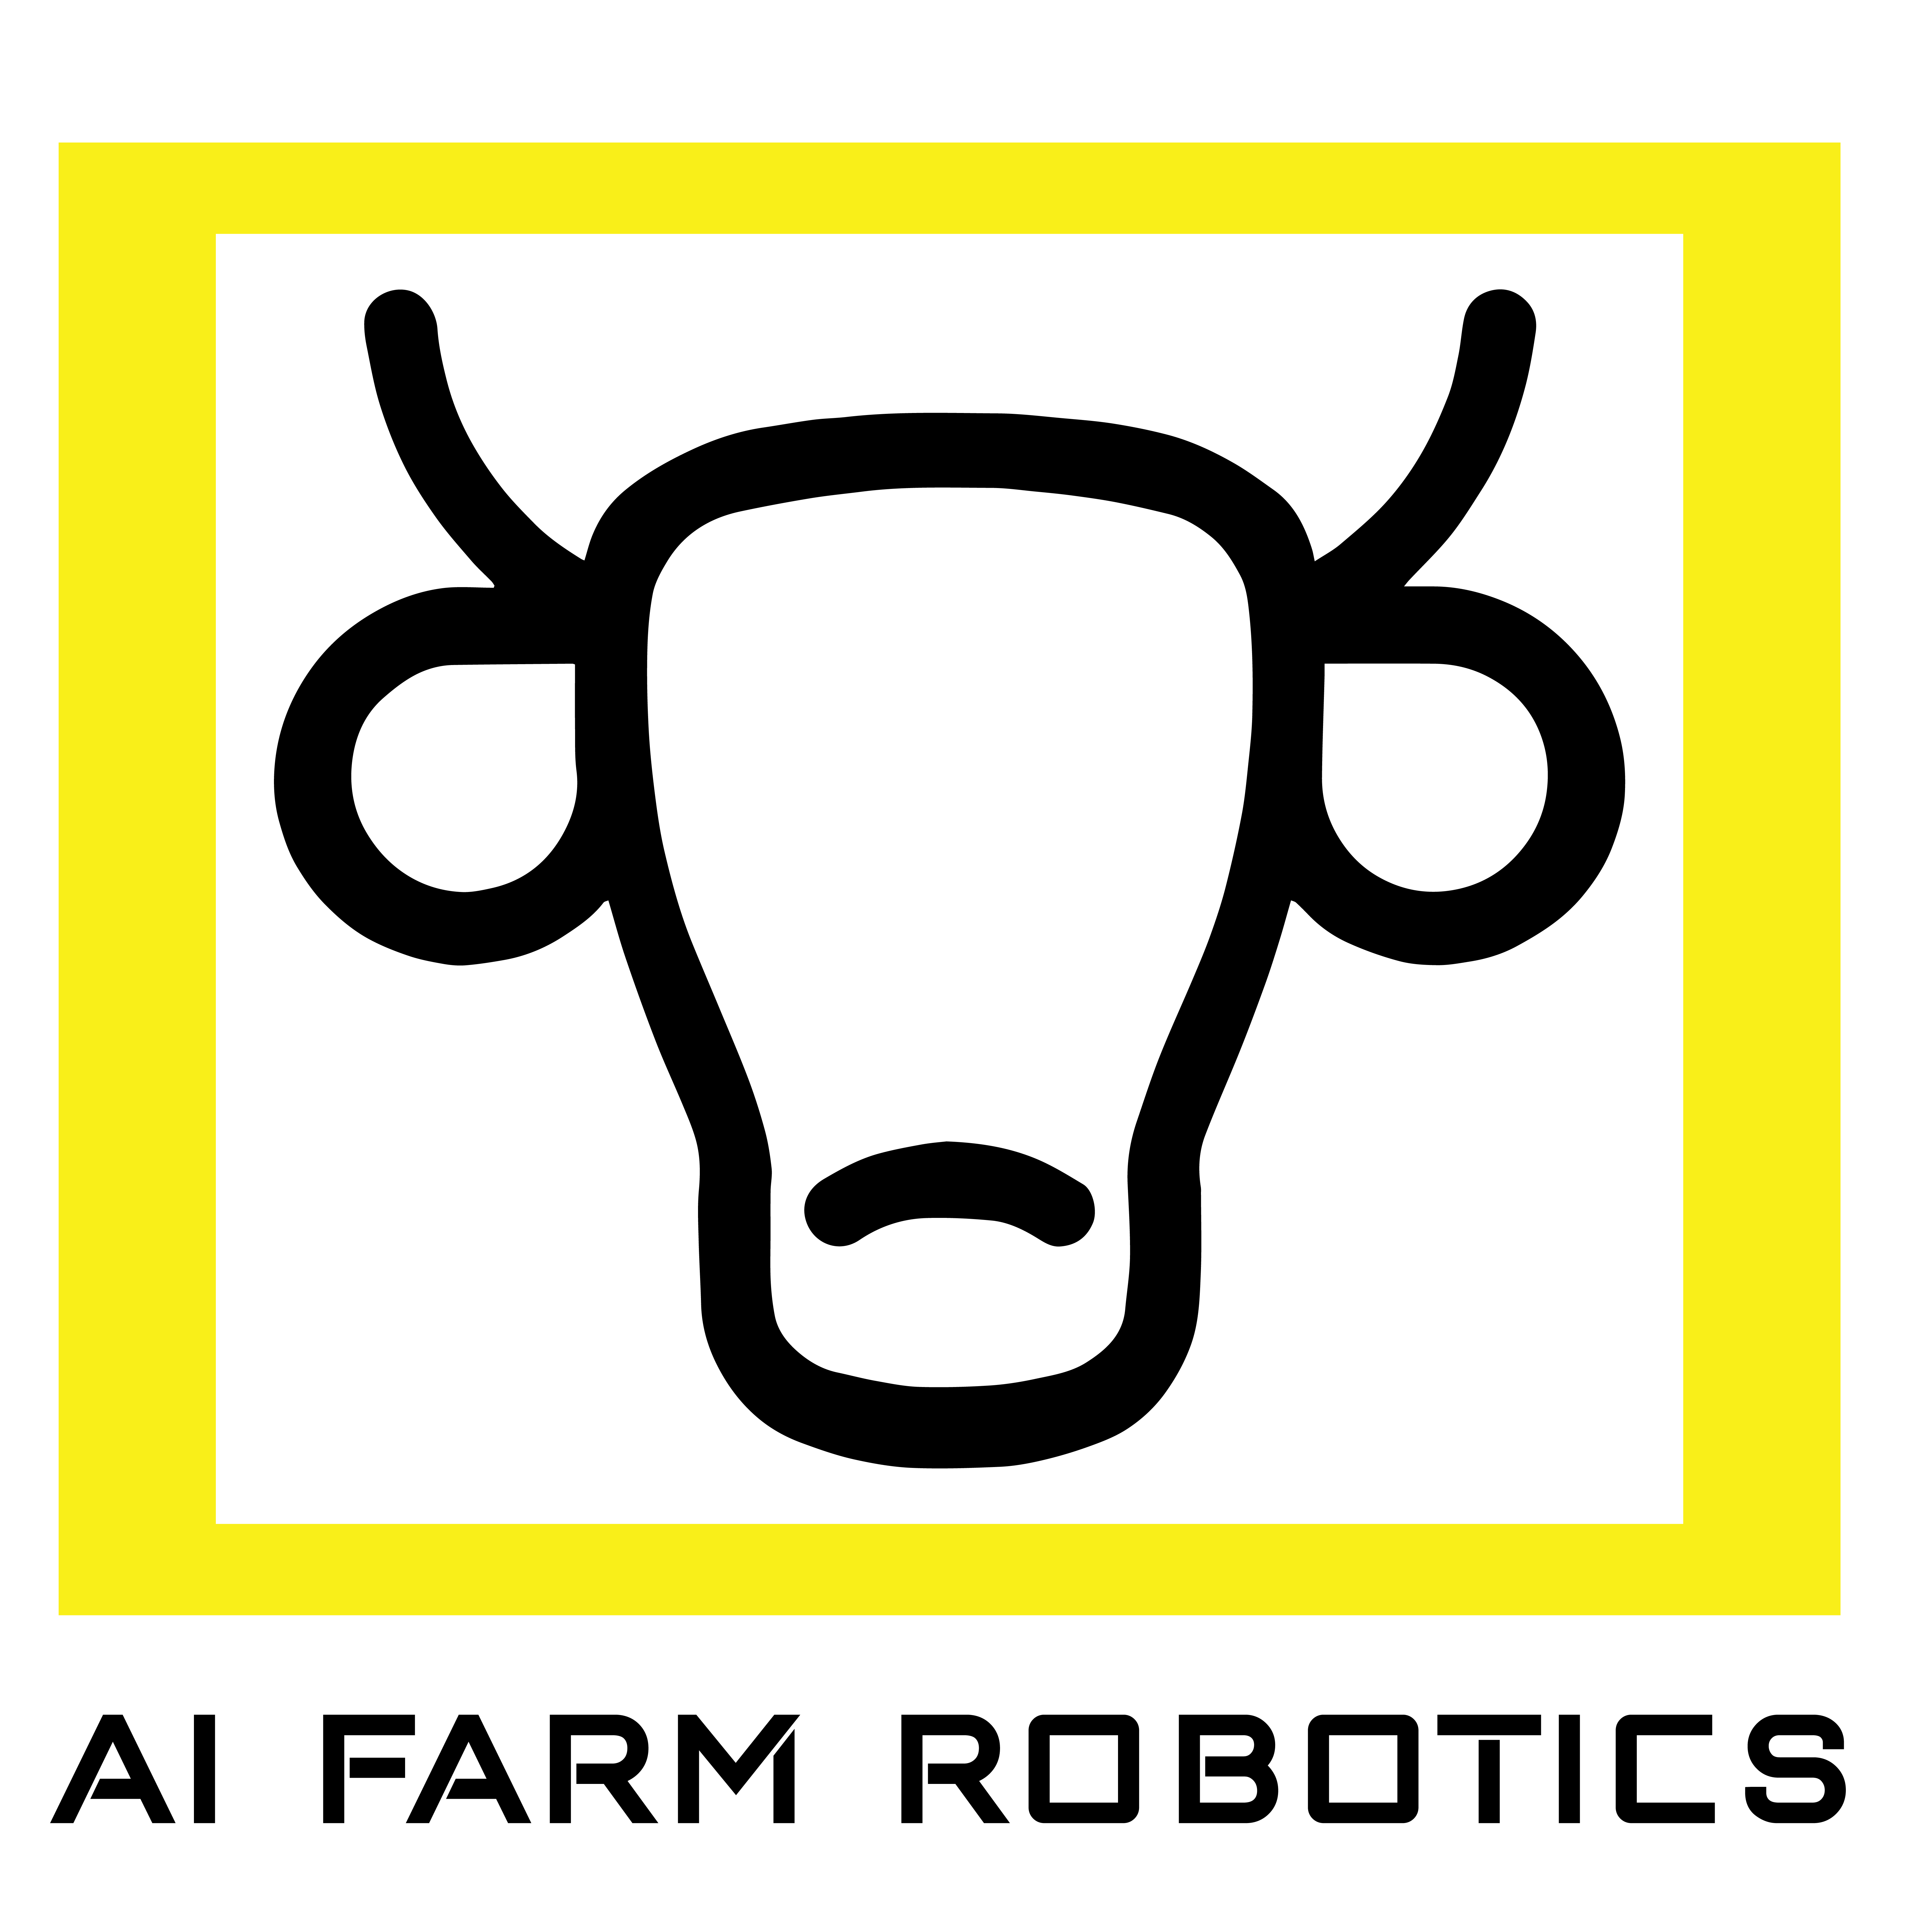
\includegraphics[width=0.5\textwidth]{figures/organization/AI-FARM.png} 
    \caption{AI Farm Robotics - Company Logo}
    \label{fig:logo}
\end{figure}

\begin{description}
    \item[Address:] AIF Business Center, First Floor (Units B12/B13), Connexion Building, Corner of Koh Pich Street and Park Ave, Koh Pich City, Phnom Penh
    \item[Tel:] +855 10 686 878
    \item[Email:] \href{mailto:info@aifarm.dev}{info@aifarm.dev}
    \item[Website:] \href{https://aifarm.dev/}{https://aifarm.dev/}
    \item[Mission:] Transform Cambodia to be a robotic Nation
    \item[Vision:] A Living Code Creator - Robot Makes Robot - GPT for Robotics
\end{description}

\subsection{Organization Services}

AI Farm Robotics Factory is a 100\% locally owned company headquartered in Phnom Penh, Cambodia. The company delivers cutting-edge technological solutions that support the digital modernization of enterprises, public institutions, and educational organizations. Its offerings are structured around four complementary pillars, addressing the needs of businesses, government bodies, and the agricultural and food sectors.

\begin{itemize}
    \item \textbf{Consulting Services}: The company designs bespoke AI and robotics strategies tailored to each client's strategic objectives, guiding organizations through the identification, planning, and adoption of intelligent technologies.
    
    \item \textbf{Engineering Solutions}: AI Farm Robotics builds physical, state-of-the-art robots and automated machines engineered to meet the specific requirements of the local market, ensuring that hardware deployments are both practical and scalable.
    
    \item \textbf{Software Solutions}: The company develops intelligent applications and machine-learning models that enhance operational efficiency, streamline workflows, and foster innovation across client operations.
    
    \item \textbf{Education \& Training}: Through partnerships with schools and universities, AI Farm Robotics establishes STEM laboratories, designs academic curricula, and trains the next generation of technology leaders, contributing to the growth of Cambodia's digital talent pipeline.
\end{itemize}
